\section{Introduction}
\begin{frame}{\insertsection}
    \begin{itemize}
        \item Industrial  data-intensive  systems  require reliability and  availability
        \item Risk of tampering with system operational data
        \item Critical errors, downtime, undefined behavior and fatal accidents
        \item Need for a controlled environment, strict access barriers
    \end{itemize}
\end{frame}

\subsection{Objective}
\begin{frame}{\insertsubsection}
    \begin{itemize}
        % \item HostSecure Concept
        \item HostSecure IDS - Data-intensive Security Management Platform
        \item Intrusion Detection and Prevention for Industrial Systems
    \end{itemize}
    
    \begin{figure}[h]
        \centering
        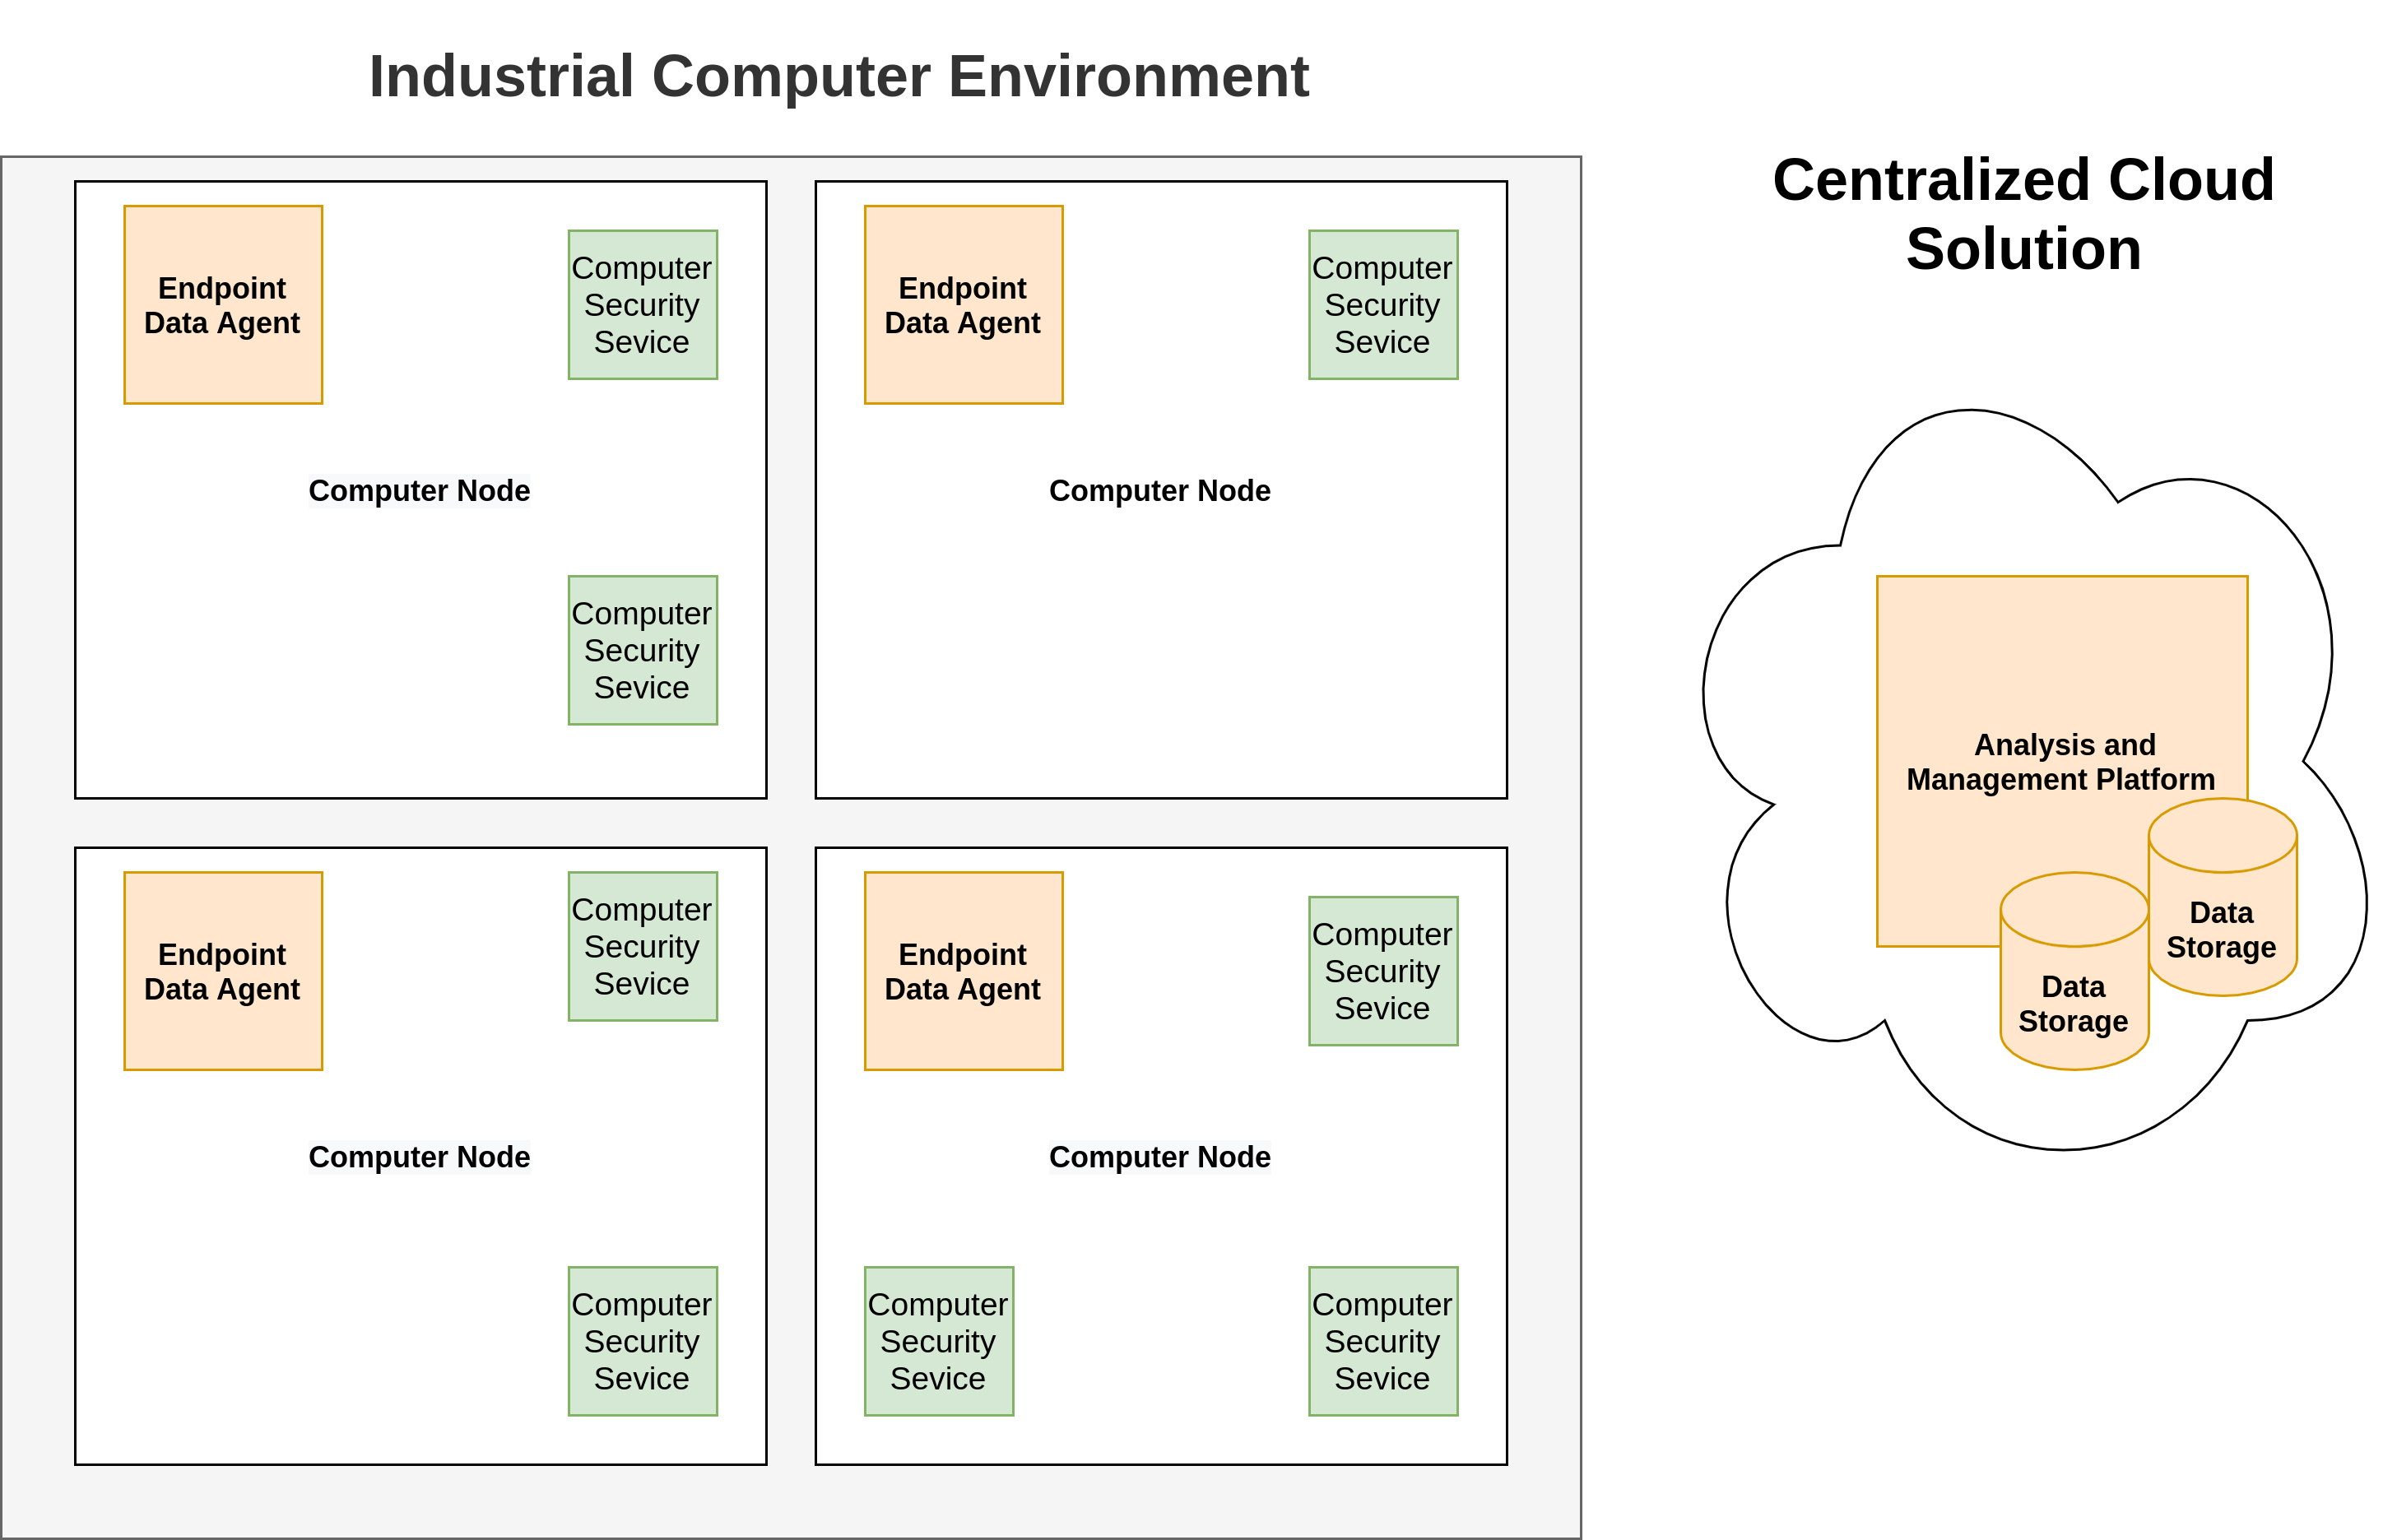
\includegraphics[width=10cm]{img/hostsecure-concept_pp.png}
        \label{fig:concept}
    \end{figure}
\end{frame}

\subsection{Development process}
\begin{frame}{\insertsubsection}
    \begin{itemize}
        \item Week 1: Research and design
        \item Week 2: Implementation
        \item Week 3: Integration and documentation
        \vspace{0.5cm}
        \item Continuous Integration, Continuous Deployment (CI/CD)
    \end{itemize}
    
    \begin{figure}[h]
        \centering
        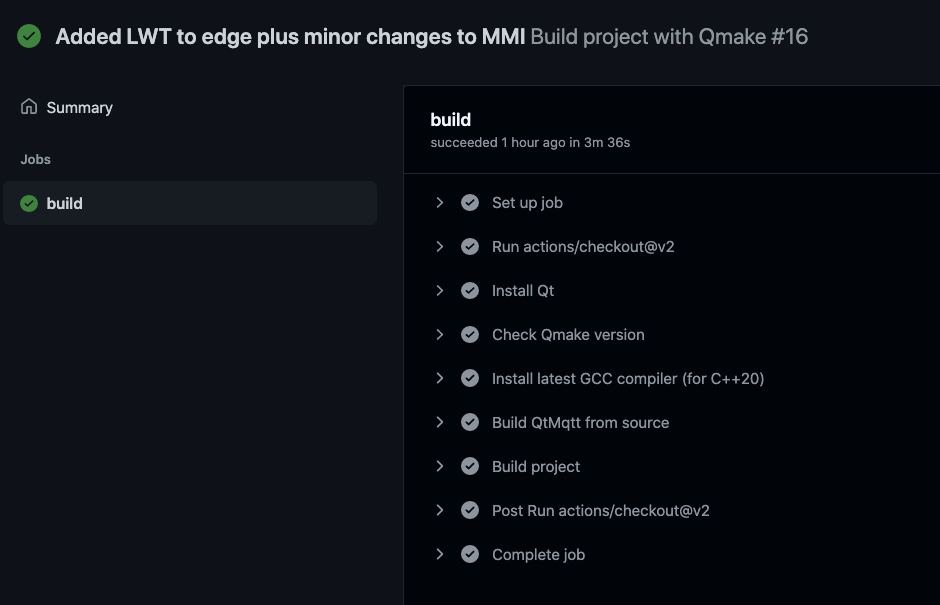
\includegraphics[width=8cm]{img/pipeline.png}
        \label{fig:concept}
    \end{figure}
\end{frame}

\subsection{Technologies, tools and standards}
\begin{frame}{\insertsubsection}
    \begin{itemize}
        \item C++ and Qt Framework
        \item Qmake and QML
        \item D-Bus
        \item USBGuard
        \item MQTT
        \item SQLite
        \item Git
    \end{itemize}
\end{frame}


\section{Systems Design and Implementation}
\subsection{Endpoint Agent}
\begin{frame}{\insertsubsection}
    \begin{itemize}
        \item Data aggregator for security services
        \item Communicate to cloud or laterally to other endpoint nodes
   \end{itemize}
    
    \begin{figure}[h]
        \centering
        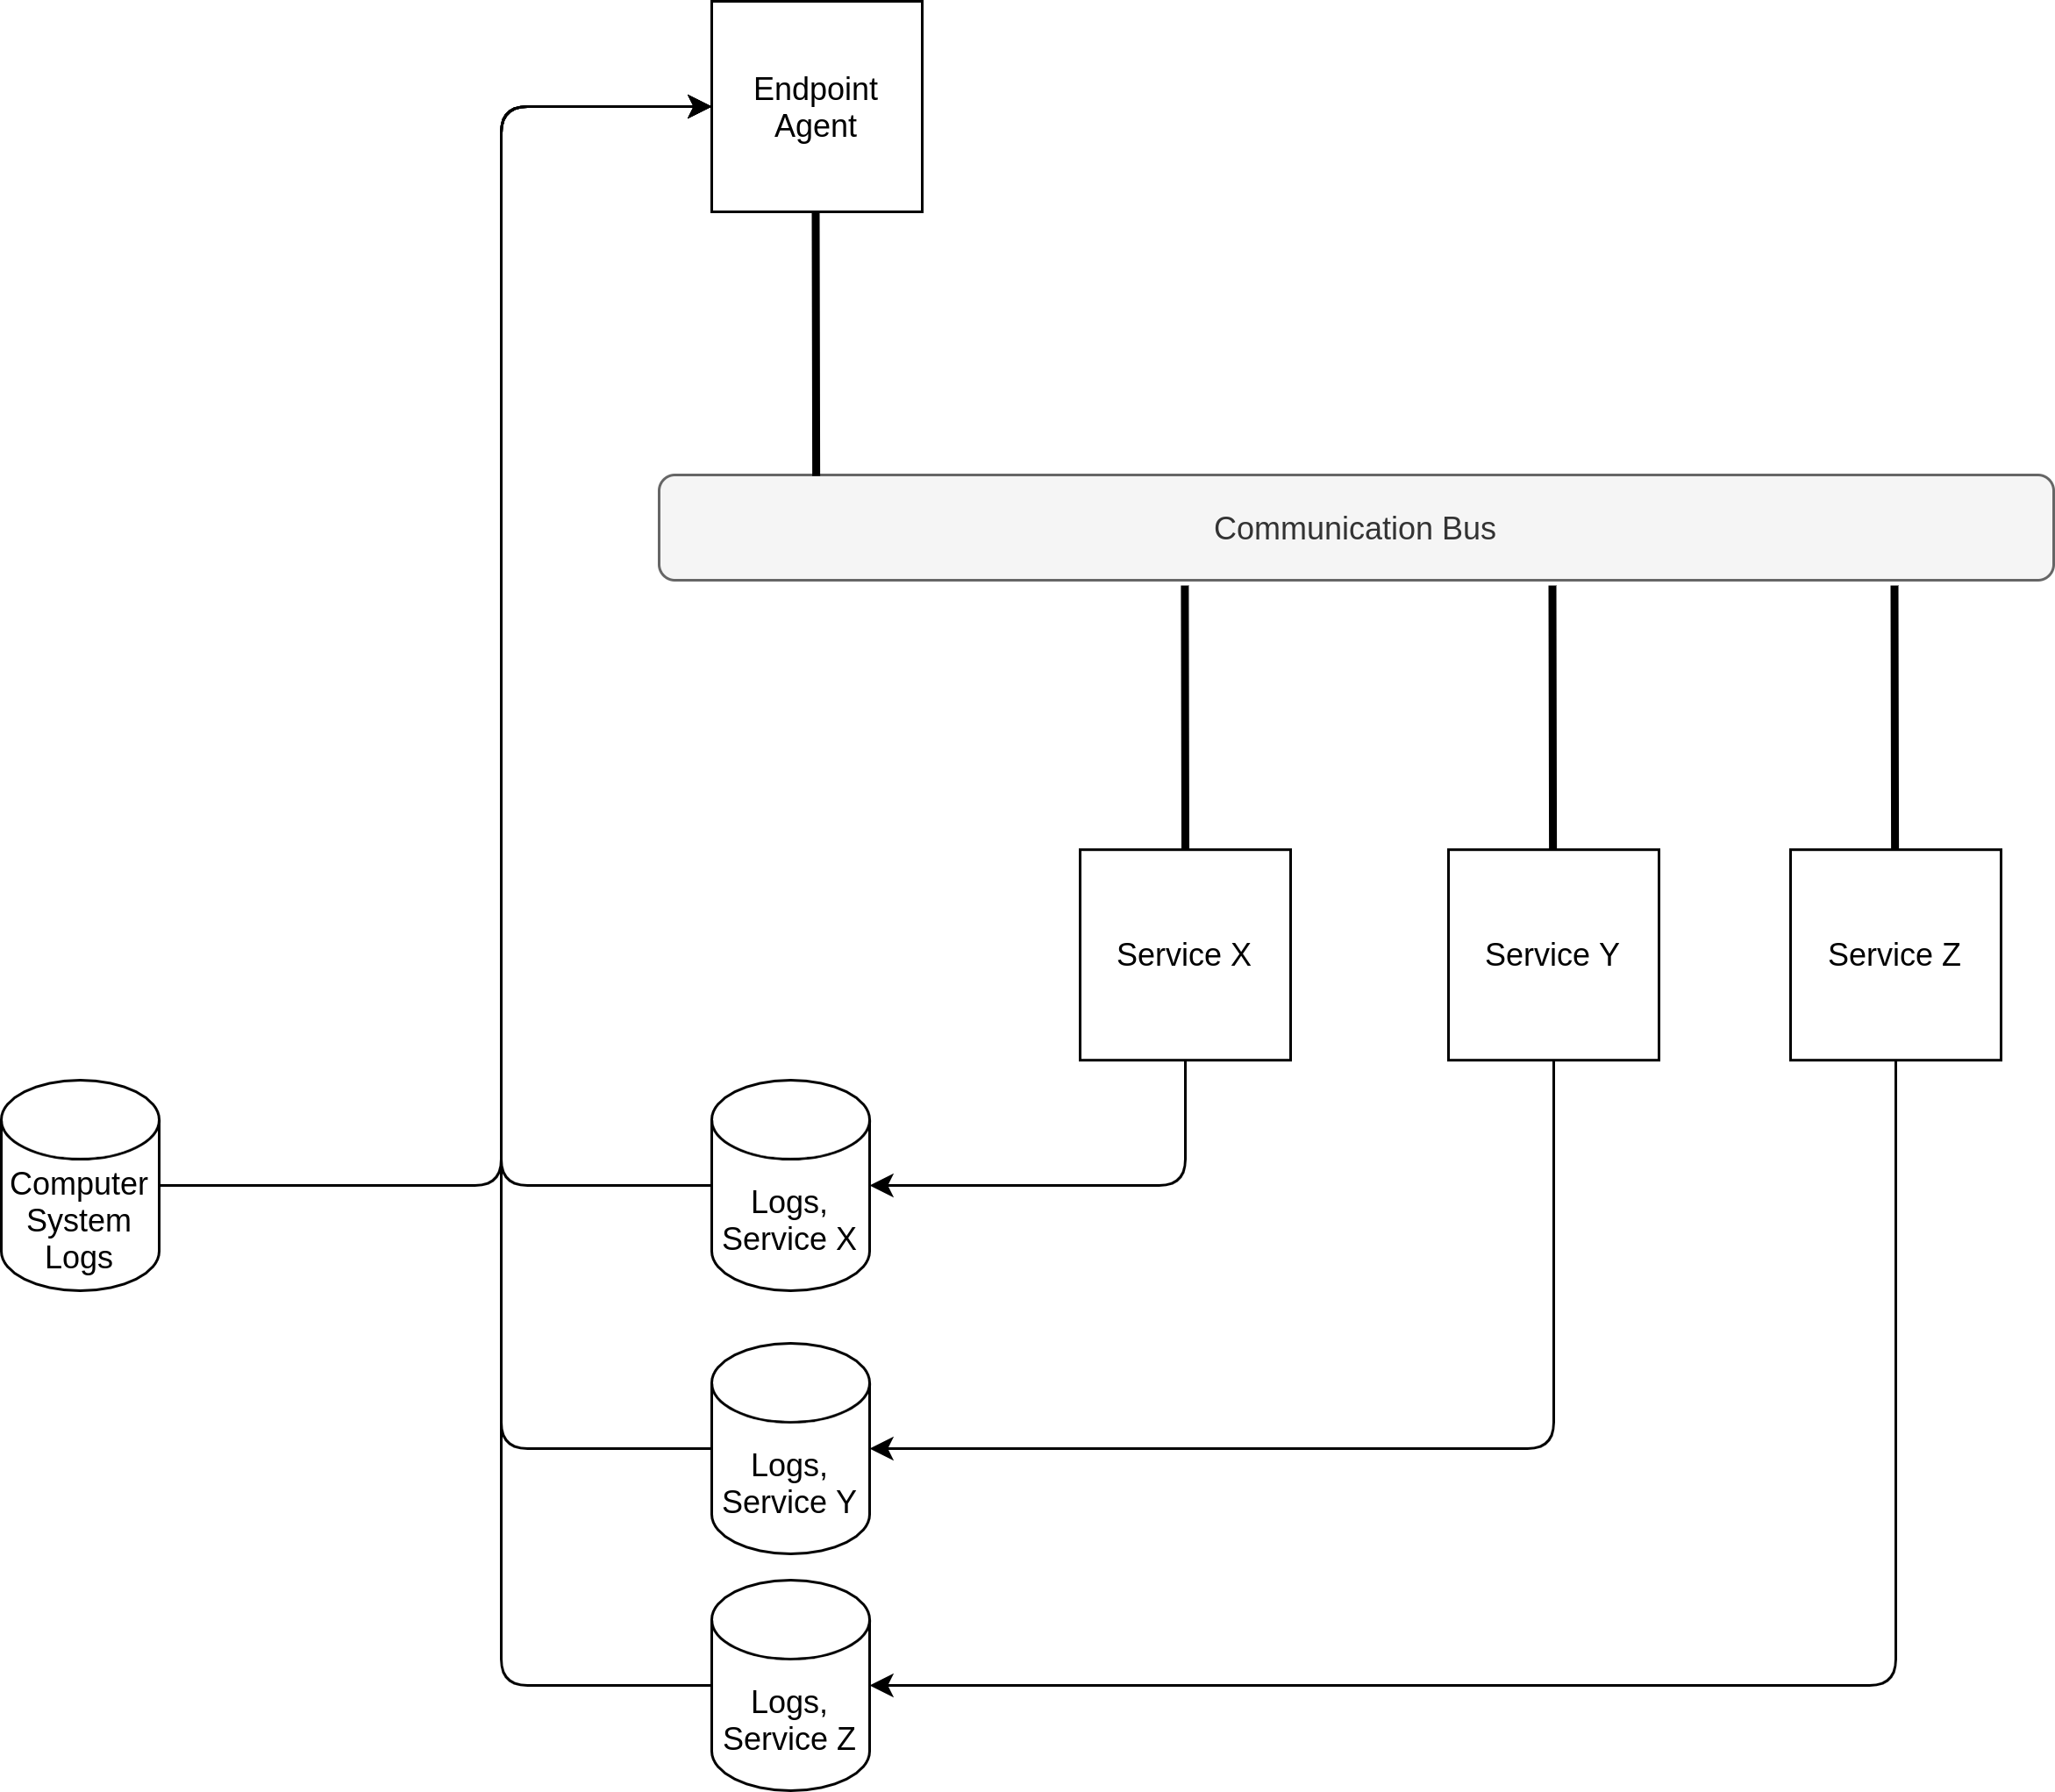
\includegraphics[width=8cm]{img/endpoint_agent_design-pp1.png}
        \label{fig:endpoint_agent_overview}
    \end{figure}
\end{frame}

\begin{frame}{Implementation}
    \begin{itemize}
        \item Qt D-BUS Message Bus
        \item USB Access Security Service
    \end{itemize}
    
    \begin{figure}[h]
        \centering
        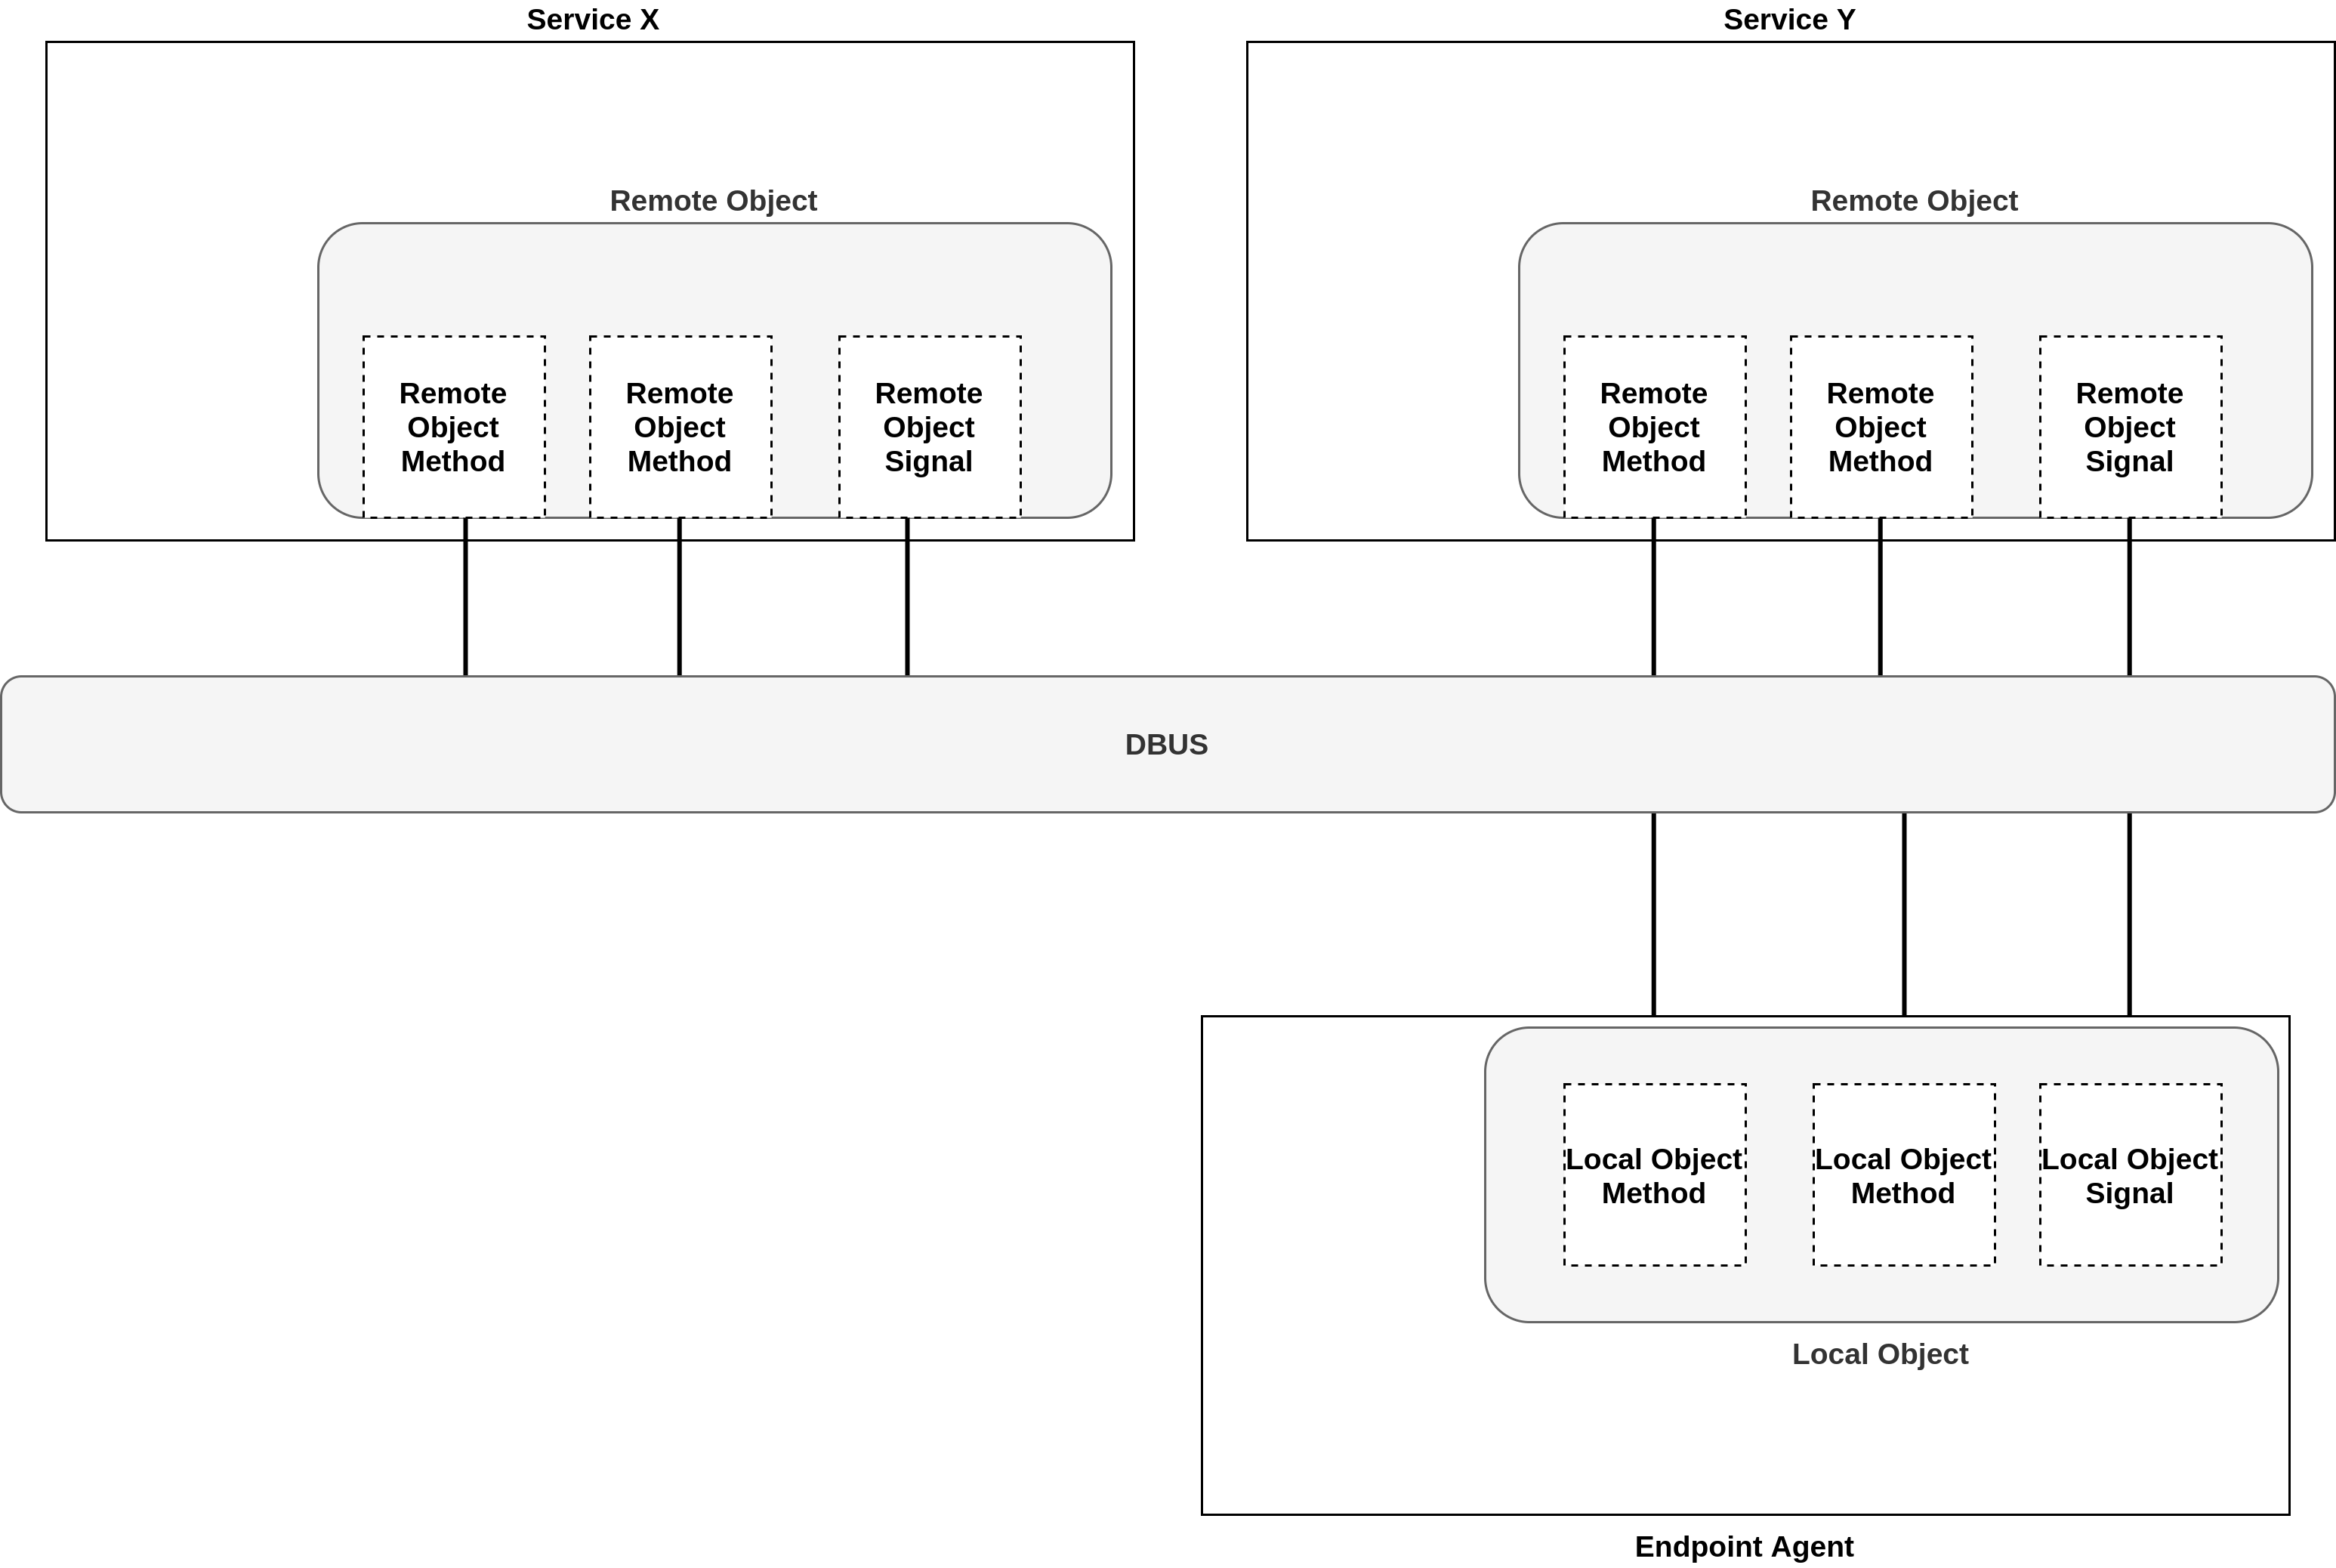
\includegraphics[width=10cm]{img/endpoint_agent_dbus_pp2.png}
        \label{fig:endpoint_agent_dbus}
    \end{figure}
\end{frame}

\subsection{Connectivity and Network Communications}
\begin{frame}{\insertsubsection}
    \begin{itemize}
        \item MQTT messaging protocol
        \item Machine-to-machine (M2M) communication
        \item Publish-subscribe messaging architecture
    \end{itemize}
    
    \begin{figure}[h]
        \centering
        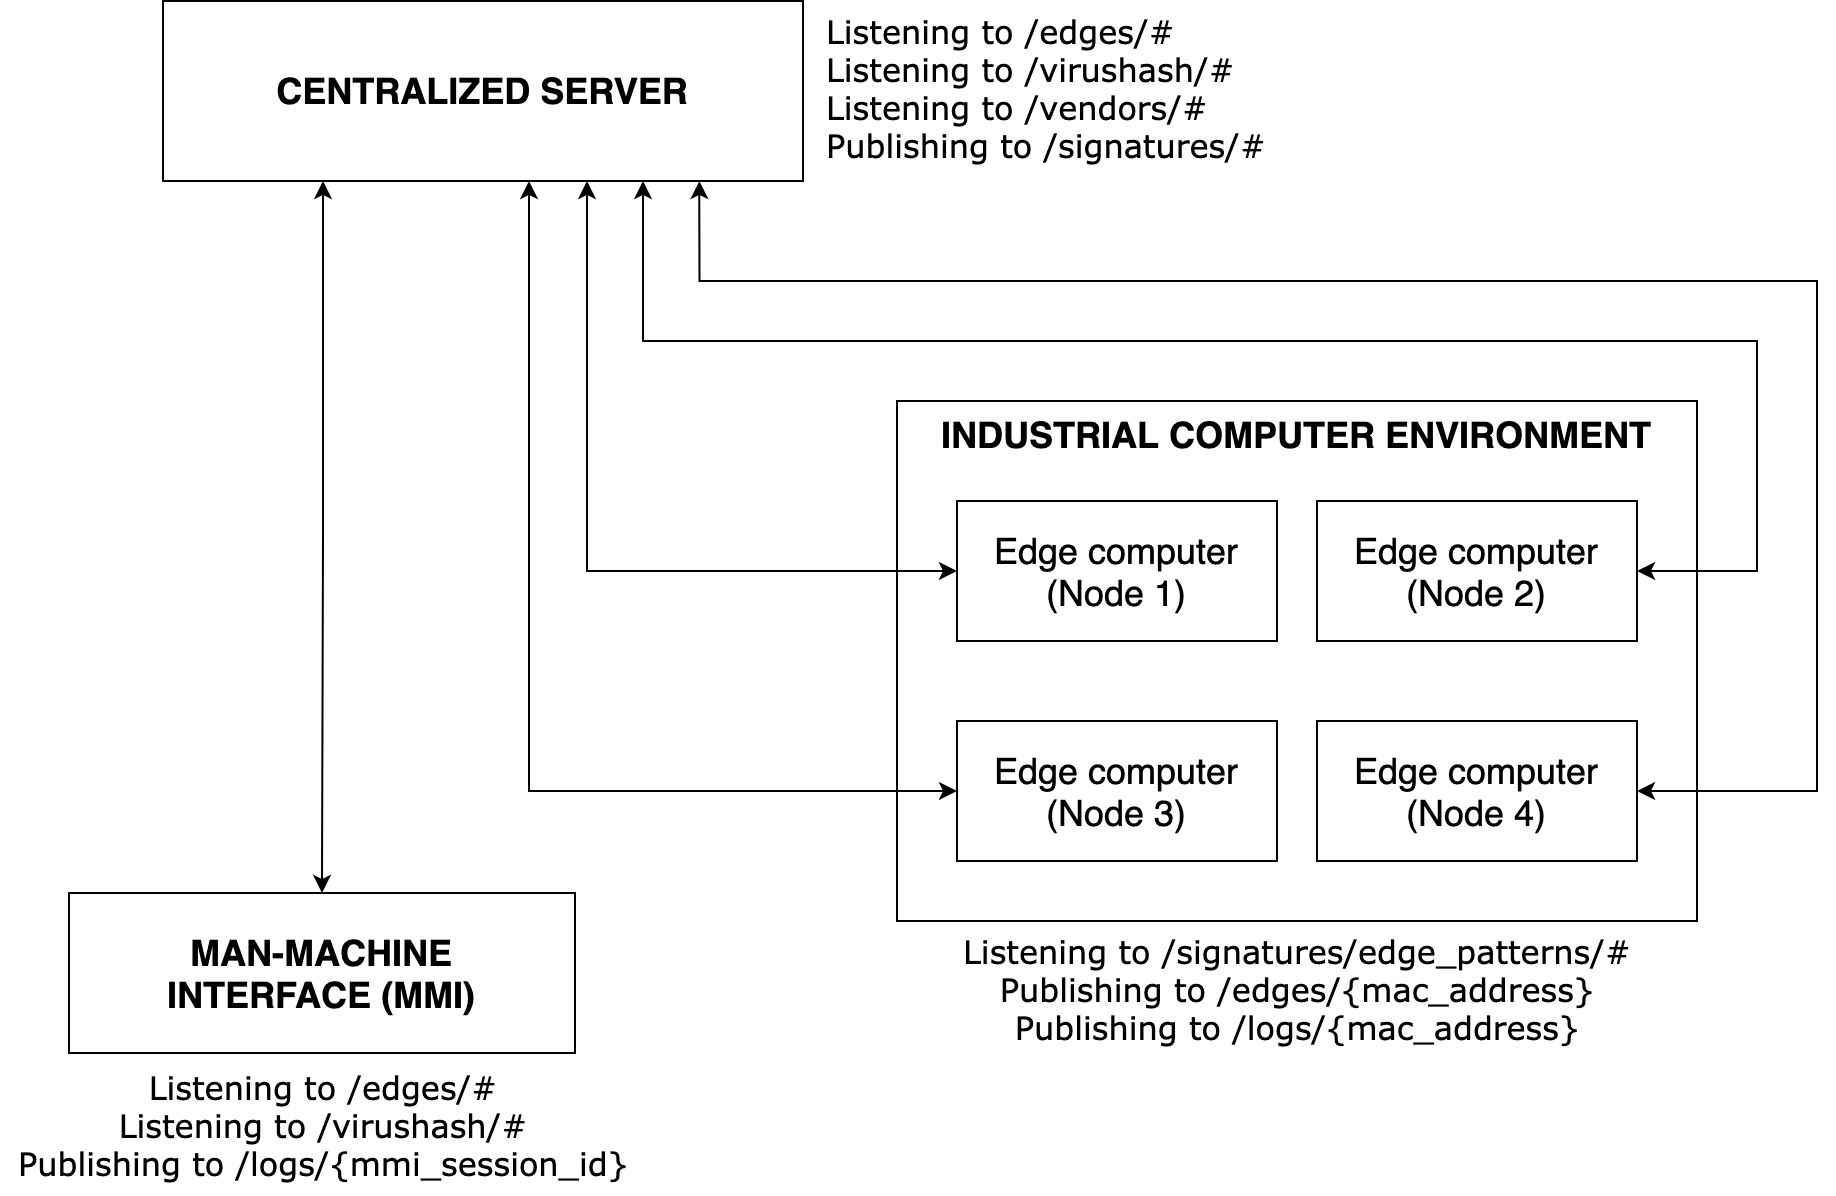
\includegraphics[width=9cm]{img/mqtt_diagram.png}
        \label{fig:mqtt_diagram}
    \end{figure}
\end{frame}

\begin{frame}{\insertsubsection}
    \begin{itemize}
        \item Publish/subscribe to various topics
        \item Highly scalable messaging architecture
    \end{itemize}
    
    \vspace{0.5cm}
    \begin{center}
        \begin{tabular}{ | l | l | p{6cm} |}
        \hline
        \textbf{Type} & \textbf{Topic} & \textbf{Description} \\ \hline
        Repository & /virushash/\# & Repository for all virus hashes \\ \hline
        Repository & /products/\# & Repository for all products \\ \hline
        Repository & /edges/\# & Repository for all edge computers \\ \hline
        Action & /edges/\{mac-address\}/new-edge & Register a new edge computer \\ \hline
        Action & /edges/\{id\}/heartbeat & Send a heartbeat signal to broker \\ \hline
        ... & ... & ... \\ \hline
        \end{tabular}
    \end{center}
\end{frame}

\subsection{Man-machine Interface (MMI)}
\begin{frame}{\insertsubsection}
    \begin{itemize}
    
        \item Qt Framework, C++ and QML
        \item Security Management Platform
        \item Create custom rules
        \item Last Will and Testament
    \end{itemize}
        \begin{figure}[h]
        \centering
        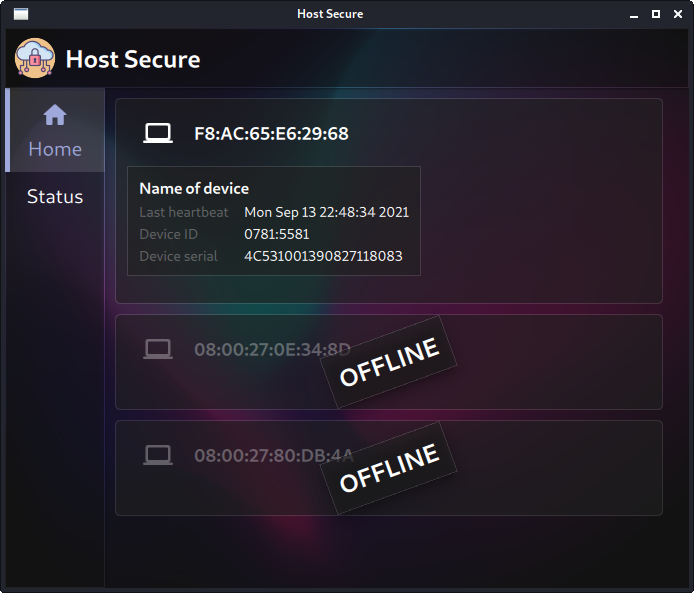
\includegraphics[width=8cm]{img/mmi_home.png}
        \label{fig:db_erdiagram}
    \end{figure}
    
\end{frame}


\begin{frame}{\insertsubsection}
    \begin{figure}[h]
        \centering
        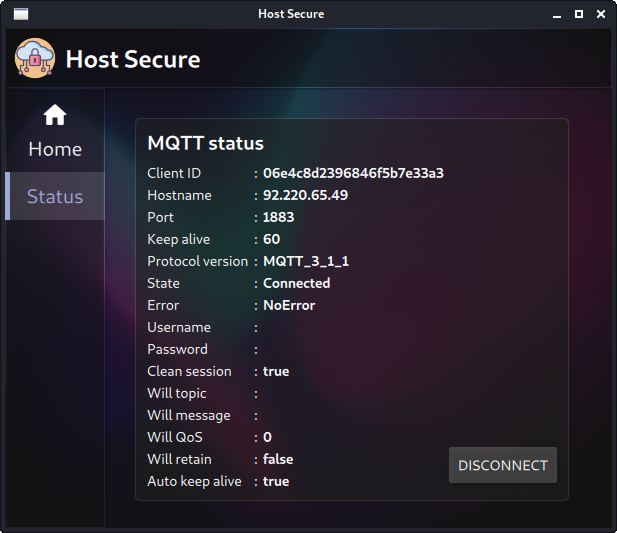
\includegraphics[width=8cm]{img/mmi_status.png}
        \label{fig:db_erdiagram}
    \end{figure}
\end{frame}

\subsection{Database and Storage}
\begin{frame}{\insertsubsection}
    \begin{itemize}
        \item SQLite
        \item Qt Framework plugins/drivers
        \item DatabaseHandler API and DatabaseMqttClient
    \end{itemize}
    
    \begin{figure}[h]
        \centering
        \includegraphics[width=8cm]{img/database_ERdiagram.png}
        \label{fig:db_erdiagram}
    \end{figure}
\end{frame}



\subsection{Data Management and Analysis}
\begin{frame}{\insertsubsection}
    \begin{itemize}
        \item Inspect and model the data collected from all endpoints
        \item Jupyter Notebook and Python
        \vspace{0.5cm}
        \item Future directions and improvements are extensive
        \begin{itemize}
            \item Machine learning to predict new anomaly patterns and signatures
            \item Generate new rules based on human behaviour
            \item Improve the intrusion detection model of our system
        \end{itemize}
    \end{itemize}
\end{frame}

\begin{frame}{\insertsubsection}
    \begin{itemize}
        \item Preview:
    \end{itemize}
    
    \begin{figure}[h]
        \centering
        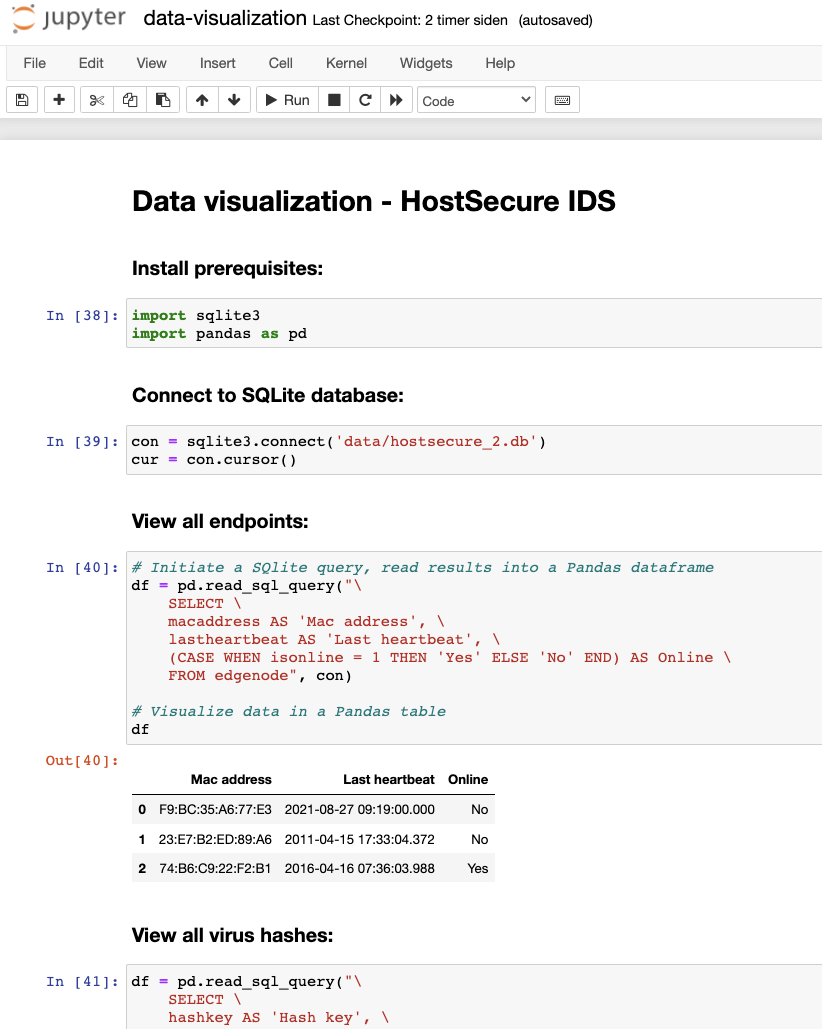
\includegraphics[width=6cm]{img/jupyter.png}
        \label{fig:db_erdiagram}
    \end{figure}
\end{frame}


\section{Demonstration}
\begin{frame}{\insertsection}
    \begin{itemize}
        \item Example Flow: USB Device :)
    \end{itemize}
      \begin{figure}[h]
        \centering
        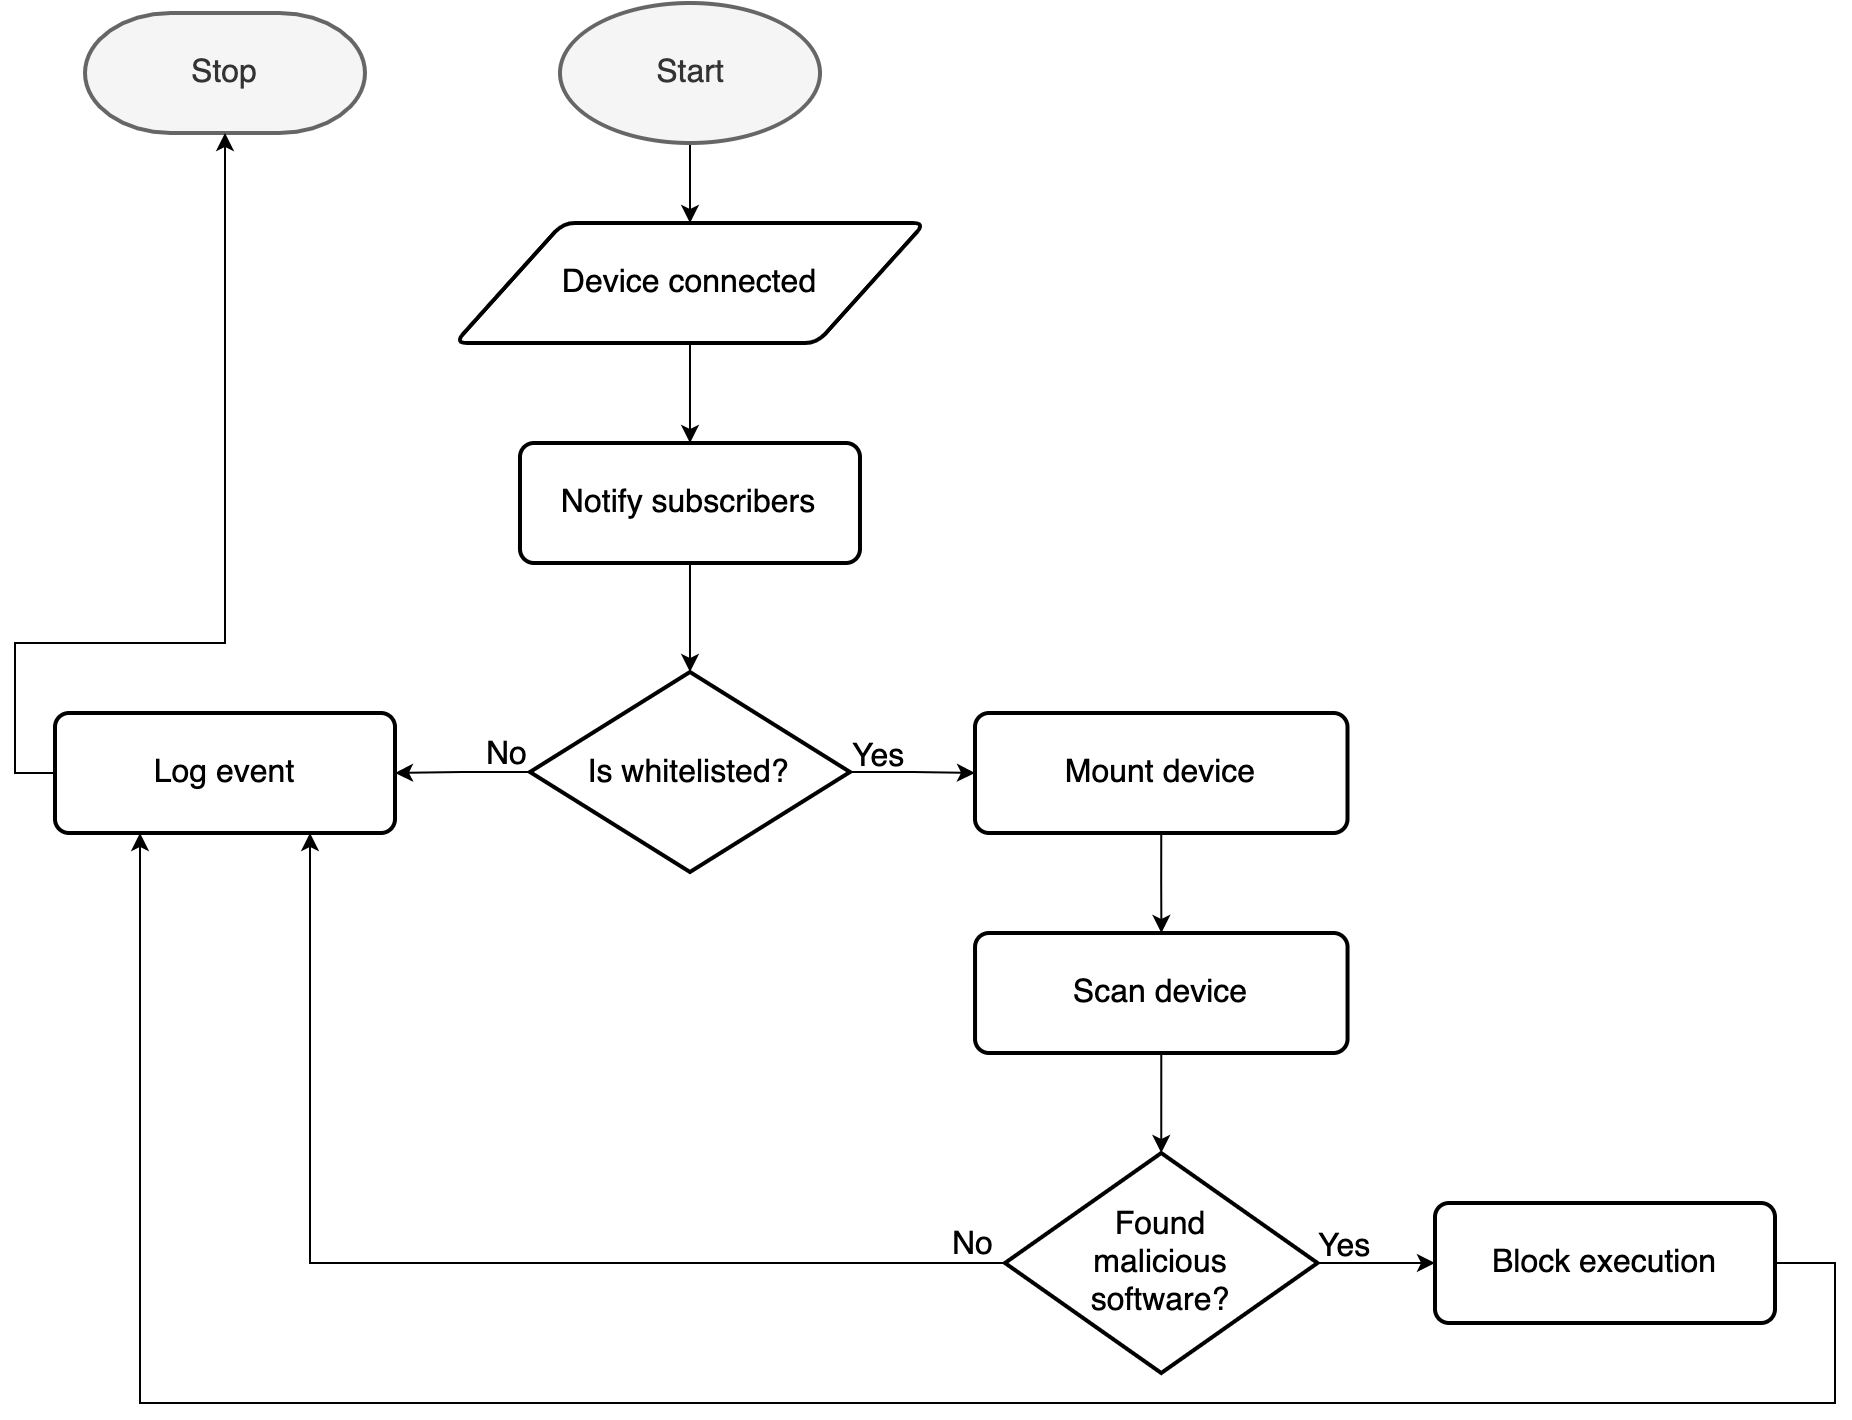
\includegraphics[width=9cm]{img/flow_pp.png}
        \label{fig:example_flow}
    \end{figure}
\end{frame}
